% Makros zur Kompatibilitaet mit Onlinemodul: 
 \providecommand{\MoIl}[1][]{\mbox{}#1]\mathopen{}} 
 \providecommand{\MoIr}[1][]{#1[\mbox{}} 
 \providecommand{\MIntvlSep}{;} 
 \providecommand{\MElSetSep}{\, ; \, } 
 \begin{MAufgabe}{Lineare Betrags(un)gleichungen}{vr, 2016, MaTeX}
L\"osen Sie die Gleichung
$$
 \MDS 5\left| 3\, x \right|+2\, x + 3=  \left|  - x - 1 \right| +2\, x
$$  

\ifLsg\MLoesung

Im ersten Schritt k\"onnen die Terme au\ss{}erhalb der Betragszeichen zusammengefasst werden:

\begin{align*} 
 5\left| 3\, x \right|+2\, x + 3=  \left|  - x - 1 \right| +2\, x\\ 
\Leftrightarrow15\, \left|x\right| - \left|x + 1\right| + 3= 0 
 \end{align*}

F\"ur diese Gleichung haben wir 4 F\"alle zu unterscheiden: 
\begin{enumerate}
\item $ \MDS 
\begin{cases} 
 0 \leq 3\, x\\ 
0 \leq  - x - 1
 \end{cases}
 \mbox{ : keine L\"osung. Diese Bedingung ist nirgendwo erf\"ullt.}$ 
\item $ \MDS 
\begin{cases} 
 0 \leq 3\, x\\ 
 - x - 1 < 0
 \end{cases}
\Leftrightarrow 0 \leq x\Leftrightarrow x \in [ 0 \, \MIntvlSep \, \infty\MoIr $ 
\item $ \MDS 
\begin{cases} 
 3\, x < 0\\ 
0 \leq  - x - 1
 \end{cases}
\Leftrightarrow x \leq -1\Leftrightarrow x \in \MoIl  -\infty \, \MIntvlSep \, -1]$ 
\item $ \MDS 
\begin{cases} 
 3\, x < 0\\ 
 - x - 1 < 0
 \end{cases}
\Leftrightarrow x < 0 \wedge -1 < x\Leftrightarrow x \in \MoIl  -1 \, \MIntvlSep \, 0\MoIr $ 
\end{enumerate} 
Der 1. Fall ist nirgendwo erf\"ullt. Betrachte weiter nur die restlichen F\"alle.
 
 Fallunterscheidung: 

 \begin{enumerate} 
 \item Sei $ \MDS x\in[ 0 \, \MIntvlSep \, \infty\MoIr $. 
 In diesem Fall gilt: 
  $ \MDS \left| 3\, x\right|=3\, x$ und $ \MDS \left|  - x - 1\right|=x + 1$. \\ 
 Damit ist die Gleichung 
 $$ 
15\, \left|x\right| - \left|x + 1\right| + 3= 0
$$
 \"aquivalent zur Gleichung
 $$ 
5\left(3\, x\right)-\left( x + 1\right)+3= 0 
$$  
$$ 
 \Leftrightarrow 14\, x + 2= 0 
$$  
$$ \Leftrightarrow x = - \frac{1}{7} . 
 $$ 
 Die L\"osung muss auch die Fallbedingung $x\in [ 0 \, \MIntvlSep \, \infty\MoIr  $ erf\"ullen. Die gefundene L\"osung $x=- \frac{1}{7}$ erf\"ullt die Fallbedingung  $x\in [ 0 \, \MIntvlSep \, \infty\MoIr $ nicht und deshalb ist  $$
 \mathcal{L}_{1}=\emptyset 
 $$ 
\item Sei $ \MDS x\in\MoIl  -\infty \, \MIntvlSep \, -1]$. 
 In diesem Fall gilt: 
  $ \MDS \left| 3\, x\right|=- 3\, x$ und $ \MDS \left|  - x - 1\right|= - x - 1$. \\ 
 Damit ist die Gleichung 
 $$ 
15\, \left|x\right| - \left|x + 1\right| + 3= 0
$$
 \"aquivalent zur Gleichung
 $$ 
5\left(- 3\, x\right)-\left(  - x - 1\right)+3= 0 
$$  
$$ 
 \Leftrightarrow 4 - 14\, x= 0 
$$  
$$ \Leftrightarrow x = \frac{2}{7} . 
 $$ 
 Die L\"osung muss auch die Fallbedingung $x\in \MoIl  -\infty \, \MIntvlSep \, -1] $ erf\"ullen. Die gefundene L\"osung $x=\frac{2}{7}$ erf\"ullt die Fallbedingung  $x\in \MoIl  -\infty \, \MIntvlSep \, -1]$ nicht und deshalb ist  $$
 \mathcal{L}_{2}=\emptyset 
 $$ 
\item Sei $ \MDS x\in\MoIl  -1 \, \MIntvlSep \, 0\MoIr $. 
 In diesem Fall gilt: 
  $ \MDS \left| 3\, x\right|=- 3\, x$ und $ \MDS \left|  - x - 1\right|=x + 1$. \\ 
 Damit ist die Gleichung 
 $$ 
15\, \left|x\right| - \left|x + 1\right| + 3= 0
$$
 \"aquivalent zur Gleichung
 $$ 
5\left(- 3\, x\right)-\left( x + 1\right)+3= 0 
$$  
$$ 
 \Leftrightarrow 2 - 16\, x= 0 
$$  
$$ \Leftrightarrow x = \frac{1}{8} . 
 $$ 
 Die L\"osung muss auch die Fallbedingung $x\in \MoIl  -1 \, \MIntvlSep \, 0\MoIr  $ erf\"ullen. Die gefundene L\"osung $x=\frac{1}{8}$ erf\"ullt die Fallbedingung  $x\in \MoIl  -1 \, \MIntvlSep \, 0\MoIr $ nicht und deshalb ist  $$
 \mathcal{L}_{3}=\emptyset 
 $$ 
 \end{enumerate} 
  Die L\"osungsmenge des Ausgangsproblems ist die Vereinigung der einzelnen L\"osungsmengen: 
$$ \mathcal{L} = \mathcal{L}_{1} \cup \mathcal{L}_{2} \cup \mathcal{L}_{3} 
 = \emptyset\cup \emptyset\cup \emptyset 
   =\emptyset 
   . $$ 
 
 \begin{center}
 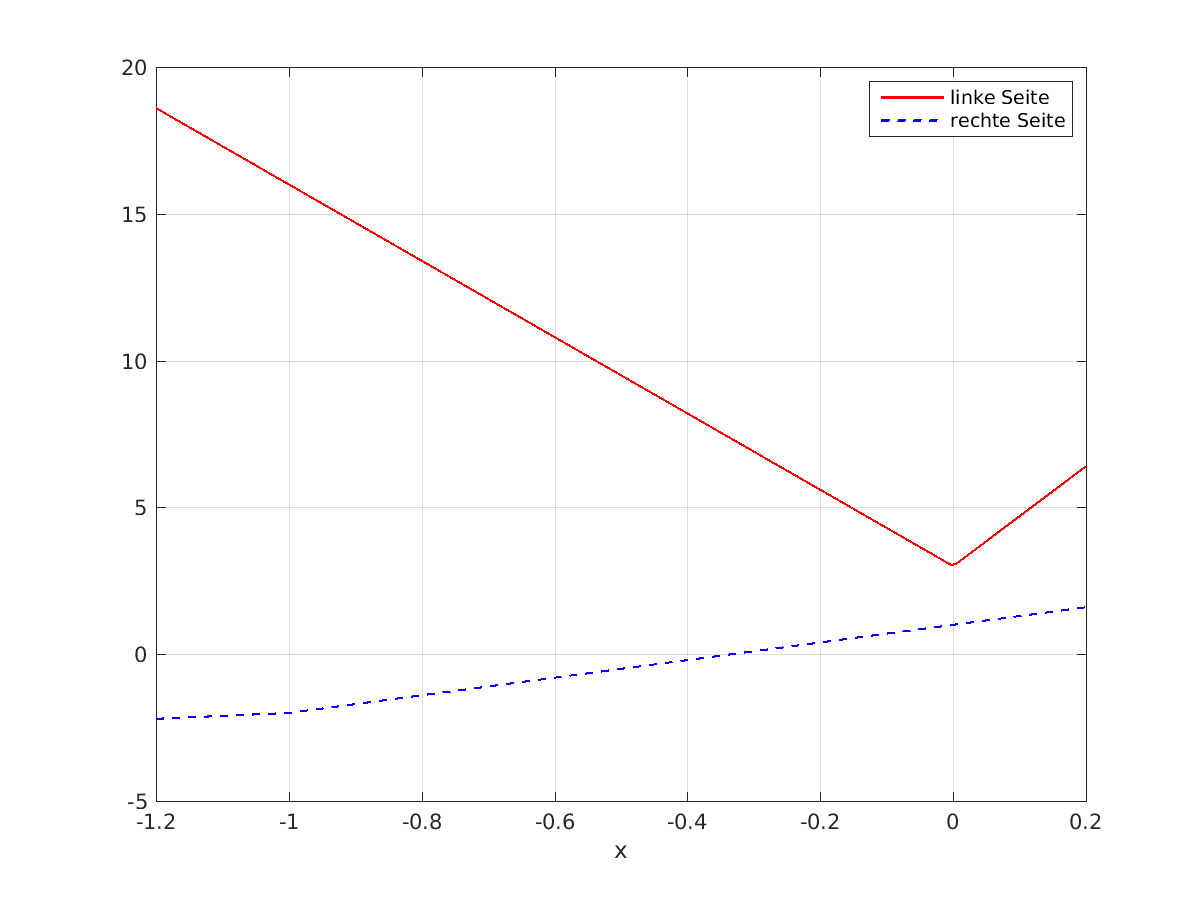
\includegraphics[width=0.8\linewidth]{Abb_zur_Ag_autogenerated_ineq_8.png} \end{center}
 
\else\relax\fi
 \end{MAufgabe}